\section{Conceitos Básicos}

\subsection{Introdução}


% \subsection{Problema criação de um sistema}
Suponha que estamos num país em que não haja energia elétrica e desejamos
definir um plano de implantação para suprir a necessidade de energia
dos seus habitantes que pararam no século XIX. Para ser feita de forma eficiente, esta tarefa requer, de início, conhecimento acerca da demanda por energia dos habitantes e dos custos para atender esta demanda.

O primeiro passo é estimar qual é a demanda por energia nesse país.
Mas não basta um plano contendo apenas a demanda imediata; a expansão do sistema deve ser prevista preferencialmente com décadas de antecedência. E este é apenas o primeiro passo de uma série de etapas que compõe o planejamento de um sistema elétrico. As etapas são as seguintes: 
\begin{itemize}
\item Planejamento de capacidade
\item Definição dos custos de produção
\item Planejamento do estoque de recursos hídricos
\item Definição dos recursos a serem utilizados dadas as restrições
\item Despacho econômico (ou quanto a usina irá produzir de forma a minimizar os custos totais)
\item Fluxo de potência
\item Proteção e estabilidade do sistema
\end{itemize}

O diagrama apresentado na figura \ref{fig:Horizontes-de-planejamento} mostra as diferentes etapas relacionando com seus horizontes de planejamento, e seu nível de detalhamento. Nota-se que quanto menor o horizonte de tempo, maior deve ser o nível de detalhamento necessário para a correta operação. Por exemplo, não faz sentido discutir despacho econômico quando lidamos com projetos de instalação de novas usinas para aumento da capacidade.

\begin{figure}[h]
\begin{centering}
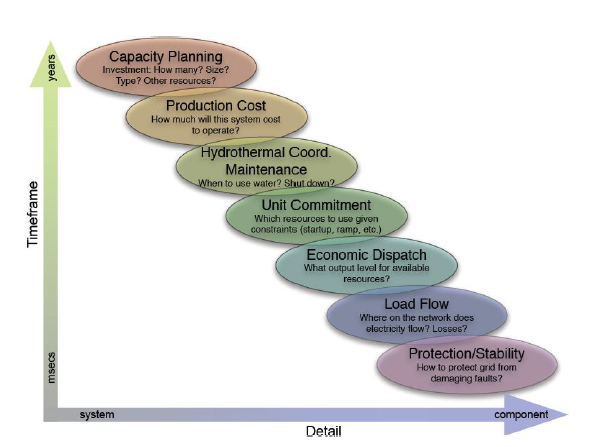
\includegraphics[scale=1]{anexos/hor-plan}
\par\end{centering}

\caption{\label{fig:Horizontes-de-planejamento}Horizontes de planejamento}
\end{figure}



Uma vez definida a demanda a atender, devemos escolher qual tipo de
usina implantar. Existem diversos tipos, como eólica, hidrelétrica,
nuclear, termelétrica (a gás, a carvão), entre outras. Além das diferenças
regionais entre a disponibilidade dos recursos naturais, há ainda
diferenças nas relações entre o custo de investimento inicial e o
custo de geração da energia. Por exemplo, uma usina termelétrica possui
geralmente um custo inicial menor que uma hidrelétrica, porém o custo
de geração da segunda é menor. A melhor solução a ser adotada possivelmente
passa pela utilização de uma combinação de diversos tipos, alguns
com custo de geração baixo mas altos investimentos iniciais para estarem
sempre ligados, e outros com baixos investimos iniciais mas alto custo
de geração para cobrir picos de demanda. Outras variáveis importantes,
além do custo das usinas, são a sazonalidade dos recursos e o tempo
de inicialização e desligamento de uma usina. O custo da operação do sistema de energia, incluindo todas suas restrições, também deve ser determinado. Para isso, é necessário realizar
o planejamento operacional, que observa horizontes menores e inclui,
por exemplo, o despacho econômico das usinas e a gestão de recursos
hídricos. 


Pode-se perceber que existem muitas variáveis envolvidas, custos desconhecidos,
e incertezas dos mais diversos tipos que afetam o funcionamento do
sistema, como a situação política do oriente médio ou até mesmo o
fenômeno El Niño. Considerar todas as variáveis ao mesmo tempo para
definir as quantidades ótimas, em qualquer estágio do planejamento,
requer um esforço computacional imenso, além de saber utilizar modelos estatísticos e utilizar métodos de mensuração de risco. Isso torna o estudo de métodos
de otimização um pré-requisito essencial para fazer uma boa gestão
de qualquer empresa que opera no mercado de energia.

Mas no que se consiste exatamente o mercado de energia?

% \subsection{Mecanismo de mercado}

Assim como no país fictício citado anteriormente, em todos os países a implantação inicial
da rede elétrica foi coordenada pela mesma instituição:
no caso, o governo. Isso mudou quando o Chile implantou o primeiro mercado de energia, em 1972, em que empresas vendiam a energia produzida por elas para as distribuidoras, por um preço determinado pelo mercado. Até então, todas as etapas do diagrama apresentado acima eram controladas pelo estado.
Assim, ao invés de ter um processo físico coordenando quanto cada empresa produz, é possível coordenar as quantidades fornecidas através da definição dos preços.
Caso os preços definidos sejam bem calibrados e não haja imperfeições
de mercado, é possível mostrar que as usinas fornecerão energia na
quantidade necessária, tal como uma empresa verticalmente integrada
faria dando ordens de produção para suas subsidiárias. Assim, estabelece-se
a fundamentação teórica para a criação de um mercado de energia.

Tal mercado tem vantagens e desvantagens. O mercado cria um ambiente competitivo e inovador que a longo e médio prazo pode conquistar avanços tecnológicos relevantes. Entretanto, um mercado mal formulado pode levar a uma competição desenfreada que pode levar ao não cumprimento de contratos e à falta de energia. 

Um exemplo interessante é o caso dos EUA e do Canadá, que possuem uma abordagem mista com relação à adoção de mercados de energia, em que cada estado ou província pode ou não adotar um esquema de mercado de energia. Na figura \ref{fig:mercado-eua}, está indicado em cores diferentes os diferentes mercados de energia existentes. Aqueles que possuem cores fracas não implementaram um mercado de energia, sendo o estado ou a província o responsável por fazer o planejamento e informar a quantidade produzida por cada produtor. Historicamente, nos EUA os mercados foram sendo implantados em alguns estados e passaram a ser adotados pelos estados vizinhos (um deles, o grupo Midwest ISO, conseguiu avançar para o Canadá, na província de Manitoba), após ter havido sucesso em suas implementações.  

\begin{figure}
\begin{centering}
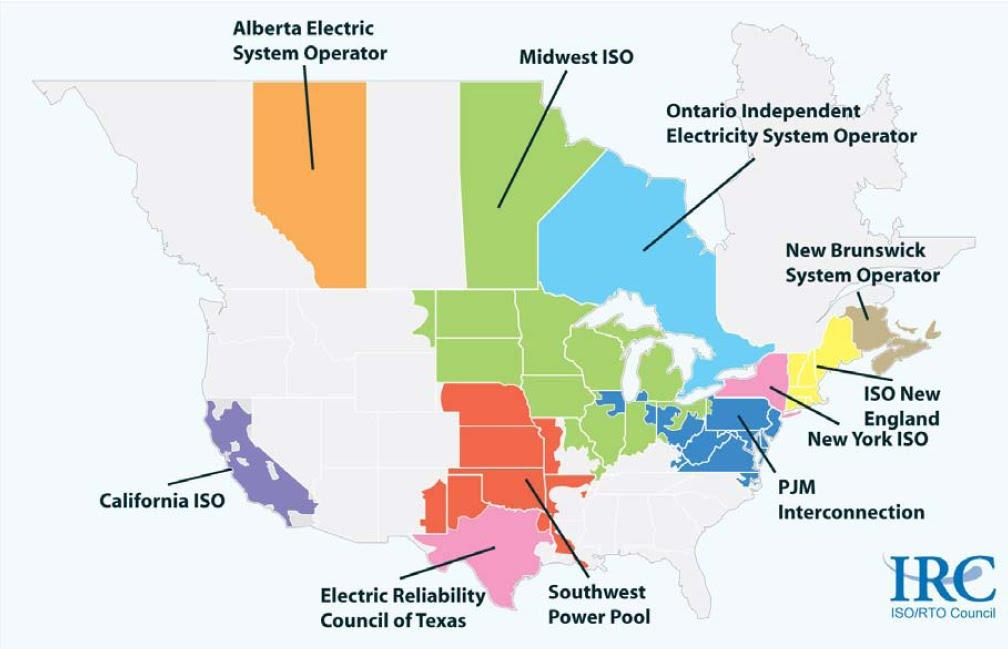
\includegraphics[scale=0.4]{anexos/mercados-eua.png}
\par\end{centering}

\caption{\label{fig:mercado-eua}A existência ou não de mercados de energia são definidos estado a estado nos EUA}
\end{figure}


Já as etapas de distribuição e transmissão são consideradas como monopólios
naturais. Entende-se por monopólio natural mercados que necessitam de
investimentos iniciais muito elevados e custos marginais muito baixos
e, com isso, a existência de concorrência poderia tornar impraticável
a existência de empresas que desejassem ofertar o serviço. Com isso,
é eficiente um esquema em que apenas uma empresa oferece o serviço
e este é regulamentada pelo governo. 

Faz parte do escopo deste trabalho, também, entender como oferecer os incentivos para que o mercado opere de forma eficiente. Se em um dado momento os atores não forem remunerados de forma adequado, gera-se um desincentivo para que novas empresas decidam entrar no negócio, diminuindo a competição e piorando a eficiência do mercado em médio prazo. 



%\subsection{Abertura do mercado no brasil}

\todo[inline]{incluir algo sobre a história da energia elétrica no brasil após a aula deste assunto}

O Brasil, assim como toda a América Latina, possui um alto percentual de usinas hidrelétricas em sua matriz energética. A figura \ref{fig:hidro-america-sul} mostra o percentual que essas usinas representam para cada país que possui mercado, assim como a existência ou não de um mercado de energia. 
Como mencionado anteriormente, a dependência de recursos hídricos (e de renováveis em geral) gera uma complexidade a mais para lidar quando planejamos o despacho das usinas. Para as usinas que possuem represa, é possível controlar seu estoque de água (até certo limite, claro) e decidir quando gerar energia com o que está no reservatório. No entanto, a quantidade de chuva em cada período é extremamente difícil de ser prevista. 
Podemos fazer decisões de consumo num período $t$ contando com chuva em $t+1$, mas se essa chuva não vir é possível que tenhamos que demandar uma alta quantia de energia de um tipo de usina mais custoso, como a termelétrica. Nesse e em outros casos, se faz necessária a mensuração do risco que corremos ao fazer decisões e não tomar decisões que possam colapsar o sistema com certa probabilidade. 


\begin{figure}[h]
\begin{centering}
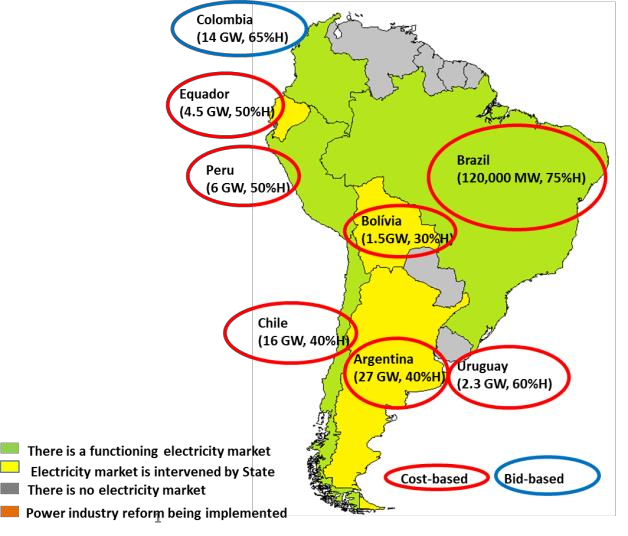
\includegraphics[scale=0.6]{anexos/hidro-america-sul.png}
\par\end{centering}

\caption{\label{fig:hidro-america-sul} Percentual de energia gerada por meio de usinas hidrelétricas e característica do mercado de energia por país}
\end{figure}


% Conclusão
Para realizar todas as atividades citadas acima, é preciso possuir
conhecimento de diversas áreas. A economia da energia elétrica é,
assim, um assunto multidisciplinar, que envolve disciplinas tão distintas
como economia, otimização, estatística, finanças e engenharia elétrica.
Uma visão global do processo de geração, assim como do funcionamento
do mercado de energia e sua interação com os consumidores, é exigida
do engenheiro elétrico do século XXI, não mais somente conhecimento
sobre capacitores e fluxos de potência. 



%%%%%%% OTIMIZAÇÃO %%%%%%%%%%%

\subsection{Revisão Otimização}
Esta sessão tem como objetivo apresentar os conceitos básicos de otimização que serão utilizados no decorrer do curso. Um modelo de otimização consiste em encontrar o valor máximo (mínimo) de uma \textbf{função objetivo}, por exemplo, o custo de geração de energia. Esta função possui um \textbf{vetor de variáveis de decisão} e é limitada por uma série de outras funções chamadas \textbf{restrições}.

Suponha que você é um dono de uma fábrica de móveis e deve decidir quais móveis produzir afim de obter o maior lucro possível. A fábrica produz armários e berços, que são representados pelas letras $A$ e $B$ respectivamente. No entanto, a quantidade produzida é limitada pelo estoque de matéria prima da fábrica, sendos estas madeira e ferro, representadas por $M$ e $F$. Sabemos que a receita líquida de um armário é de 4 reais e a do berço de 3 reais. Além disso, para se produzir um armário são necessárias 2 unidades de ferro e 1 unidade de madeira, e para o berço 1 unidade de ferro e 2 unidades de madeira. A fabrica possui 4 unidades de cada insumo em estoque. O problema pode se resumido em uma \textbf{matriz de tecnologia} apresentada na tabela \ref{tabela1}.

\begin{table}[H]
\begin{center}

\begin{tabular}{l|l|l|ll}
               & Armário & Berço & Estoque &  \\ \cline{1-4}
Ferro          & 2       & 1     & 4       &  \\ \cline{1-4}
Madeira        & 1       & 2     & 4       &  \\ \cline{1-4}
Lucro Marginal & 4       & 3     &         & 
\end{tabular}
\caption{Matriz de Tecnologia da Fábrica}
\label{tabela1}
\end{center}
\end{table}

Para encontrar o lucro ótimo devemos primeiro responder às seguintes perguntas:
\begin{itemize}
\item Quais são as variáveis de decisão do modelo?
\item Qual é a função objetivo do modelo?
\item Quais são as restrições do modelo?
\end{itemize}

A função objetivo é aquela que desejamos maximizar, no caso, o lucro. As variáveis de decisão são aquelas que devemos escolher afim de chegar ao resultado ótimo, ou seja, a quantidade produzida de cada móvel. As restrições do modelo são geradas pelas limitações do estoque. 

Formulação do problema:
\begin{itemize}
\item Variáveis de decisão: quantidade a produzir de cada produto $x_{A}$ e
$x_{B}$.
\item Função objetivo $f(x_{A},x_{B})=4x_{A}+3x_{B}$
\item Restrições:



\begin{itemize}
\item A quantidade de madeira utilizada não pode ser maior que o estoque:
$2x_{A}+1x_{B}\leq4$
\item A quantidade de ferro utilizada não pode ser maior que o estoque:
$1x_{A}+2x_{B}\leq4$
\item Não é permitido produzir quantidades negativas de armário ou berço: $x_{A}\geq0$ ,$x_{B}\geq0$\end{itemize}
\end{itemize}

Existe uma forma correta de escrever o problema acima com todas as suas informações. Em geral, é assim que você vai encontrar problemas de otimização e é assim que você deve procurar escreve-los. 

\begin{align}
    & \underset{x_A, x_B\geq0}{\text{maximizar}} \hspace{1cm} 4x_A+3x_B \label{eq1} \\
    & \text{s.a}  \hspace{2.2cm} 2x_A+x_B \leq 4; \label{eq2} \\
    &             \hspace{2.65cm} x_A+2x_B\leq 4, \label{eq3}
\end{align}

Em primeiro lugar temos a função objetivo, identificando se o problema é uma maximização ou uma minimização. É comum identificar o domínio das variáveis de decisão embaixo da palavra maximizar, neste caso, estamos dizendo que a quantidade produzida de cada móvel deve ser um número real não negativo. Entretanto, identificar o domínio e incluir as restrições $x_A, x_B \geq 0$ são exatamente a mesma coisa. 

Agora que já conhecemos o problema, temos que resolve-lo. Vamos colocar cada uma das restrições em um gráfico para entende-las melhor. 

\begin{figure}[H]
\begin{centering}
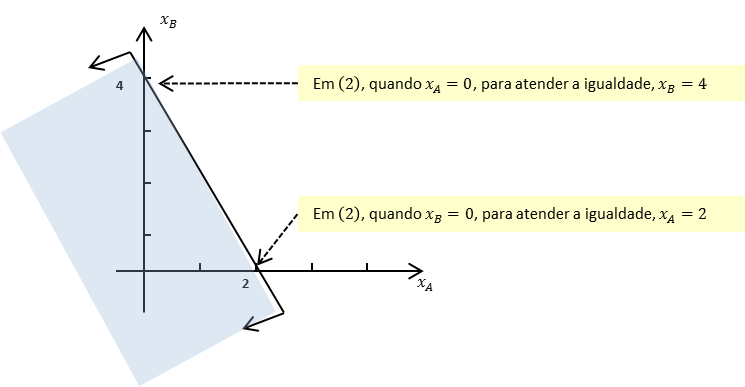
\includegraphics{pl1}\protect\caption{\label{fig:pl1}Gráfico equação (\ref{eq2})}
\end{centering}

\end{figure}

O que a figura \ref{fig:pl1} significa? No eixo $x$ temos a quantidade produzida de $x_A$ (armários), e no eixo $y$ a quantidade produzida de $x_B$ (berços). A reta desenhada na figura representa a restrição da equação \ref{eq2}. Todos os pontos a esquerda da reta são factíveis considerando apenas esta restrição. Como sabemos disso? Observe que pela restrição, se produzirmos apenas armários, a quantidade máxima produzida será 2 considerando as limitações de estoque, no caso dos berços, a quantidade será 4. Como a restrição é linear, e conheçemos dois pontos desta reta, basta ligar estes dois pontos para termos a representação gráfica da restrição.

De forma análoga, a figura \ref{fig:pl2} mostra a restrição escrita na equação \ref{eq3}.

\begin{figure}[H]
\begin{centering}
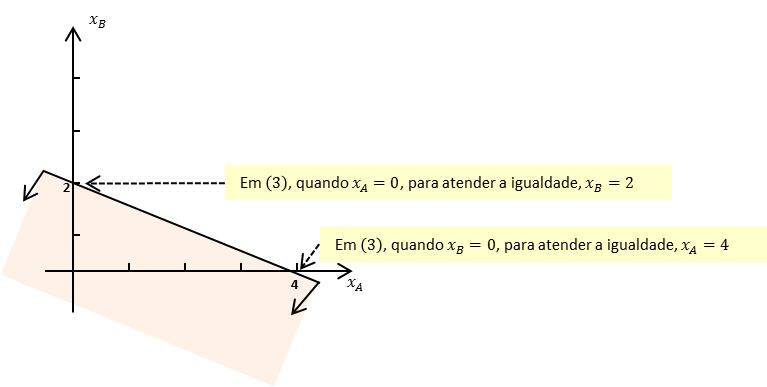
\includegraphics{pl2}\protect\caption{\label{fig:pl2}Gráfico equação (\ref{eq3})}
\end{centering}

\end{figure}

O conjunto de pontos viáveis pode ser encontrado combinando as duas figuras e levando em conta o domínio das variáveis de decisão. 

\begin{figure}[H]
\begin{centering}
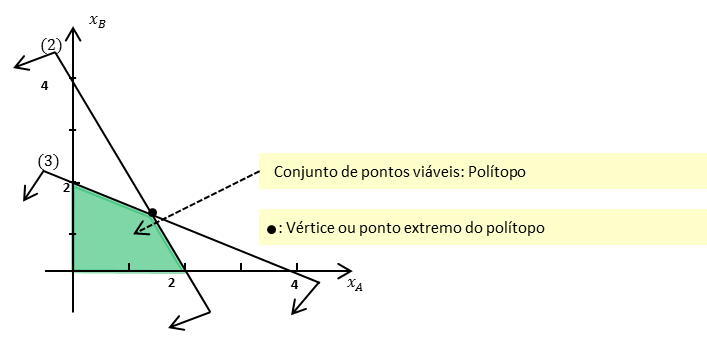
\includegraphics{pl3}\protect\caption{\label{fig:pl3}Gráfico conjunto de pontos viáveis}
\end{centering}

\end{figure}

Todos os pontos que estão na área verde da figura \ref{fig:pl3} são factíveis para a solução do nosso problema de otimização, porém apenas um deles é aquele que maximiza o lucro. Esta área é chamada de \textbf{poliedro}. Vamos encontrar qual o ponto ótimo utilizando o \textbf{gradiente}\footnote{Gradiente é o vetor das derivadas parciais da função objetivo.} da função objetivo para ver em qual direção que cresce mais rápido. Como se trata de uma função linear, o gradiente é constante e igual ao vetor $[4,3]$, representado na figura \ref{fig:pl4}.

\begin{figure}[H]
\begin{centering}
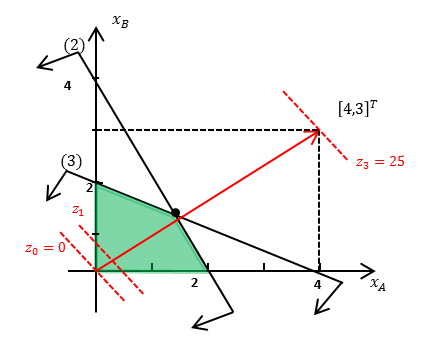
\includegraphics{pl4}\protect\caption{\label{fig:pl4}Gráfico curva de nível}
\end{centering}
\end{figure}

Com o gradiente podemos encontrar as \textbf{curvas de nível}, que são pontos onde a função objetivo tem o mesmo valor. As curvas de nível são perpendiculares ao vetor gradiente e também estão representadas na figura \ref{fig:pl4}. Finalmente, podemos resolver o problema caminhando com as curvas de nível para a direita até que ela chegue no último ponto dentro do poliedro dos pontos viáveis. 

\begin{figure}[H]
\begin{centering}
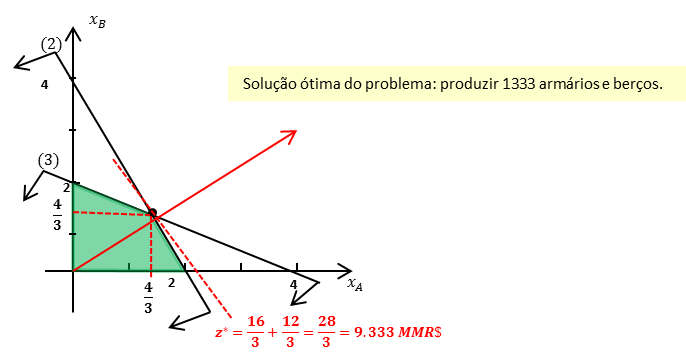
\includegraphics{pl5}\protect\caption{\label{fig:pl5}Gráfico solução ótima}
\end{centering}
\end{figure}

A figura \ref{fig:pl5} mostra a solução do problema. o Lúcro máximo é de $9.33$ reais e a solução ótima é aquela onde $x_A=x_B=\frac{4}{3}$.


Vamos colocar os passos para a resolução do problema de otimização acima em uma forma mais geral. Existem quatro passos básicos para se modelar um problema:
\begin{enumerate}
\item Compreensão do problema: 

\begin{itemize}
\item Identificar das partes relevantes o que se deseja tratar. Nesta parte,
geralmente são excluidas uma série de relações que não implicam em
uma direta, ou substancial, participação no objetivo do problema.
\end{itemize}
\item Identificação das variáveis de decisão: $x=[x_{1},...,x_{n}]^{T}$

\begin{itemize}
\item Quais são as variáveis que se deseja obter com a resolução do problema,
ou seja, o que se deseja encontrar (otimizar) e os seus respectivos
limites superiores e inferiores.
\end{itemize}
\item Identificar a função objetivo do problema: $f(x)$

\begin{itemize}
\item Especificar uma função que, dado uma possível configuração das variáveis
de decisão, reproduza o valor que se deseja maximixar ou minimixar
(otimizar): lucro, custo, confiabilidade, chance de se obter algum
resultado, distância de algum nível de referência,etc...
\end{itemize}
\item Identificar as condições que as variáveis devem atender: $g_{i}(x)\leq0$
para $i=1,...,m$

\begin{itemize}
\item Para serem válidas (viáveis) de serem escolhidas, através de inequação
ou equações.
\item É importante ressaltar que se uma possível solução não atender a alguma
das restrições, isso implica em descartar totalmente esta solução,
independentemente do valor da sua função objetivo. Logo, se existir
alguma possibilidade de discussão sobre o trade-off entre uma possível
violação e o valor da função objetivo, isso deve ser incoporado no
modelo.
\end{itemize}
\end{enumerate}

O problema do lucro ótimo da fábrica de móveis é uma \textbf{programação linear}, ou seja, tanto a função objetivo quanto as restrições são equações lineares. Todo problema de programação linear pode ser representado pela forma geral apresentada abaixo:

Forma compacta matricial
\begin{equation*}
\begin{aligned}
& \underset{x\geq0}{\text{maximizar}}
& & c^{T}x \\
& \text{s.a}
& & Ax \leq b.
\end{aligned}
\end{equation*}

Forma canônica,

\begin{equation*}
\begin{aligned}
& \underset{x}{\text{maximizar}}
& & \sum_{j=1}^{n}c_{j}\cdot x_{j} \\
& \text{s.a}
& &\sum_{j=1}^{n}a_{ij}\cdot x_{j}\leq b_{i},\qquad\forall i=1,...,m\\
& & & x_j \geq0\qquad\forall j=1,...,n.
\end{aligned}
\end{equation*}

Olhando para a forma matricial, $c$ são os coeficientes da função objetivo (4 e 3 no caso do exemplo da fábrida de móveis); $x$ são as variáveis de deicisão; $A$ é a matriz com os coeficientes das restrições; e $B$ representa o limite das restrições (no caso, o tamanho dos estoques). 
%\\

\textbf{\textit{Teoria da Dualidade}}

%\\

O \textbf{problema primal} é aquele problema que temos nas nossas mãos para resolver. Para obter algumas informações sobre o problema primal podemos utilizar o \textbf{problema dual}. No caso de uma máximização, o problema dual nos fornece um limite superior para o problema primal, se este limite superior for factível ele será o ótimo do problema primal. Isto pode ser reduzido em dois teoremas. 

\newtheorem{teo}{Teorema}[section]
\begin{teo}[Dualidade Forte]
Em um problema de programação linear, a solução ótima do problema primal será igual à solução ótima do problema dual se ambos forem viáveis. 
\end{teo}

\begin{teo}[Dualidade Fraca]
As soluções viáveis do problema dual são maiores ou iguais à solução do problema primal em um problema de maximização. No caso de um problema de minimização as relações são invertidas. 
\end{teo}


Voltando para o exemplo do problema de maximização do lucro da fábrica de móveis, lembre-se que ele era representado da seguinte forma:

\begin{align}
    & \underset{x\geq0}{\text{maximizar}} \hspace{1cm} 4x_A+3x_B \label{eq4} \\
    & \text{s.a}  \hspace{2.2cm} 2x_A+x_B \leq 4; \label{eq5} \\
    &             \hspace{2.65cm} x_A+2x_B\leq 4, \label{eq6}
\end{align}

Imagine que madeira e ferro estejam em falta no mercado, e que um comerciante deseja comprar o nosso estoque. Naturalmente, aceitaremos valores \todo{Revisar  valores de que}que, no total, sejam superiores ao nosso lucro fabricando os berços e armários. O problema do comerciante é minimizar o valor pago pelos nossos insumos levando em conta que nós só venderemos se o valor pago for maior do que o nosso lucro com a venda de berços e armários. As variáveis de decisão passam então a ser os preços dos insumos (madeira e ferro). O problema do comerciante é um problema dual do nosso problema de maximização do lucro. 

Vamos montar o problema do comerciante na forma de programação linear. A solução ótima do exemplo atende todas as restrições então, ao multiplicarmos a restrição \ref{eq4} por 3, obteremos a seguinte inequação, válida para todos os pontos viáveis.

\begin{equation}
6x_{A}+3x_{B}\leq12
\label{eq:dual1}
\end{equation}

Todos os coeficientes da desigualdade acima são maiores ou iguais do que seus respectivos coeficientes na função objetivo do problema de máximização de lucro, portanto o lucro será sempre menor do que 12.

Se fizermos uma combinação linear positiva das restrições (\ref{eq4}) e (\ref{eq5}), multiplicando-as pelo preço de cada insumo, representados por $y_A$ e $y_B$, a desigualdade será valida para todos os pontos que atendem às restrições originais:

\begin{table}[h]
\begin{center}
\begin{tabular}{lllll}
 & $y_{A}\cdot(2\cdot x_{A}+1\cdot x_{B})\leq y_{A}\cdot4$
 &  &  &  \\
 & $y_{B}\cdot(1\cdot x_{A}+2\cdot x_{B})\leq y_{B}\cdot4$ \hspace{1.0cm} + &  &  &  \\ \cline{2-2}
 & $(y_{A}\cdot2+y_{B}\cdot1)\cdot x_{A}+(y_{A}\cdot1+y_{B}\cdot2)\cdot x_{B}\leq y_{A}\cdot4+y_{B}\cdot4$ &  &  & 
 &   &  & % & 
\end{tabular}
\end{center}
\end{table}

Assumindo os valores $y_{A}=5/3$ e $y_{B}=2/3$, por exemplo, obteremos um
limite superior igual a $28/3$ , que sabemos ser o máximo do problema
da maximização do lucro. Isso nos mostra que o limite superior obtido por essa
escolha de multiplicadores resulta no menor limite possível, ou seja
, o limite ótimo. O teorema da dualidade forte garante que o GAP (diferença entre a solução dual e a primal) em problemas de otimização linear será sempre zero. Olhando para a figura \ref{fig:dualgap}

\begin{figure}[H]
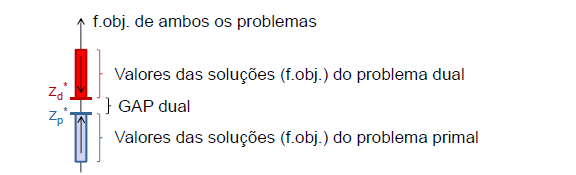
\includegraphics{pl6}\protect\caption{GAP dual}
\label{fig:dualgap}
\end{figure}


Retornando a resolução do problema em $y_{i},$ como podemos gerar
uma sistemática para encontrar os pesos de maneira que eles proporcionem
o menor limite superior (mínimo)?

Será necessário impor que cada coeficiente\footnote{Entenda como coeficiente toda a expressão que multiplica $x_A$ ou $x_B$.} da desigualdade encontrada
seja superior ao respectivo coeficiente da função objetivo : $z_{p}=4\cdot x_{A}+3x_{B}$

\begin{equation}
y_{A}\cdot2+y_{B}\cdot1\geq4
\end{equation}

\begin{equation}
y_{A}\cdot1+y_{B}\cdot2\geq3
\end{equation}

Com isso, o lado direito dessa nova desigualdade será sempre maior
que qualquer valor que a função objetivo possa valer dentro do conjunto
de pontos viáveis:

\begin{equation}
4\cdot x_{A}+3x_{B}\leq(y_{A}\cdot2+y_{B}\cdot1)\cdot x_{A}+(y_{A}\cdot1+y_{B}\cdot2)x_{B}\leq y_{A}\cdot4+y_{B}\cdot4
\end{equation}

Assim, queremos minimizar o limite superior, mexendo nos multiplicadores
$y_{i}$, sujeita a esses multiplicadores gerarem um limite superior:

\begin{align}
    & \underset{y\geq0}{\text{minimizar}} \hspace{1cm} 4y_A+4y_B \label{eq6} \\
    & \text{s.a}  \hspace{2.2cm} 2y_A+y_B \geq 4; \label{eq7} \\
    &             \hspace{2.65cm} y_A+2y_B\geq 3, \label{eq8}
\end{align}

O problema acima é um problema dual da programação linear da maximização do lucro. Ao mesmo tempo, ele é o problema do comerciante que deseja comprar nosso estoque. Ao solucionar o problema do comerciante (dual) encontramos os preços pelos quais seriamos indiferentes entre produzir móveis ou vender insumos. A figura \ref{pldual1} mostra a solução do problema dual de forma análoga à que fizemos para o problema primal. 

\begin{figure}[H]
\begin{centering}
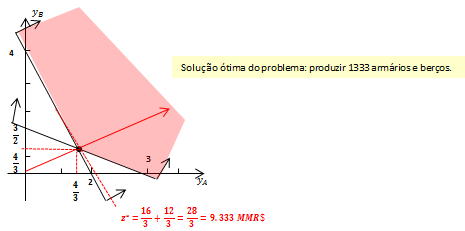
\includegraphics{pldual1}\protect\caption{\label{pldual1}Solução do problema dual}
\end{centering}
\end{figure}


De forma geral, um problema de programação linear definido como: 

\begin{equation*}
\begin{aligned}
& \underset{x\geq0}{\text{maximizar}}
& & c^{T}x \\
& \text{s.a}
& & Ax \leq b.
\end{aligned}
\end{equation*}

Tem a seguinte representação dual:

\begin{equation*}
\begin{aligned}
& \underset{y\geq0}{\text{minimizar}}
& & y^{T}b \\
& \text{s.a}
& & Ay^{T} \geq c.
\end{aligned}
\end{equation*}


\subsection{Revisão Estatística}

Otimização e estatística caminham juntas, principalmente quando estamos resolvendo problemas mais complexos. Imagine que queremos modelar um contrato de um parque eólico no ambiente livre (ACL). Para determinar o contrato, precisamos de projeções futuras da velocidade do vento, da potência gerada pelo parque e do preço da energia. Em outras palavras, precisamos gerar vários cenários possíveis para o futuro, e fazemos isto utilizando conceitos de estatística e de probabilidade. 

Como não sabemos o que vai acontecer no futuro, nossos cenários de possíveis realizações resultam em \textbf{distribuições de probabilidade}, e precisamos conhecer bem as características destas distribuições para construir cenários coerentes com a realidade. Uma distribuição de probabilidade descreve as chances de uma determinada variável assumir diferentes valores. Em outras palavras, uma distribuição é uma função que transforma valores de uma variável em probabilidade. 

Suponha que estamos jogando uma moeda. Os resultados possíveis são cara e coroa, se representarmos cara pelo número 1, e coroa por 0, temos o domínio de uma distribuição de probabilidade. A distribuição da moeda nos dirá que em $50\%$ das vezes o resultado será cara, e em $50\%$ será coroa. Esta distribuição é conhecida como \textit{distribuição de Bernoulli}.

A distribuição de Bernoulli é uma \textbf{distribuição discreta}. Em muitos casos pode ser interessante representar uma variável por uma \textbf{distribuição contínua}, ou seja, uma variável que pode assumir qualquer valor em um intervalo. A mais importante das distribuições contínuas é a \textbf{distribuição normal}. 
\\

\textbf{\textit{Distribuições Discretas}}


Já vimos que uma moeda pode ser caracterizada como uma distribuição discreta. Suponha agora que estamos jogando um dado. Ele pode assumir valores de 1 a 6 em intervalos discretos, ou seja, apenas os números inteiros de 1 a 6. A figura \ref{fig:prob1} apresenta o \textbf{histograma} de um dado. 

\begin{figure}[H]
\begin{centering}
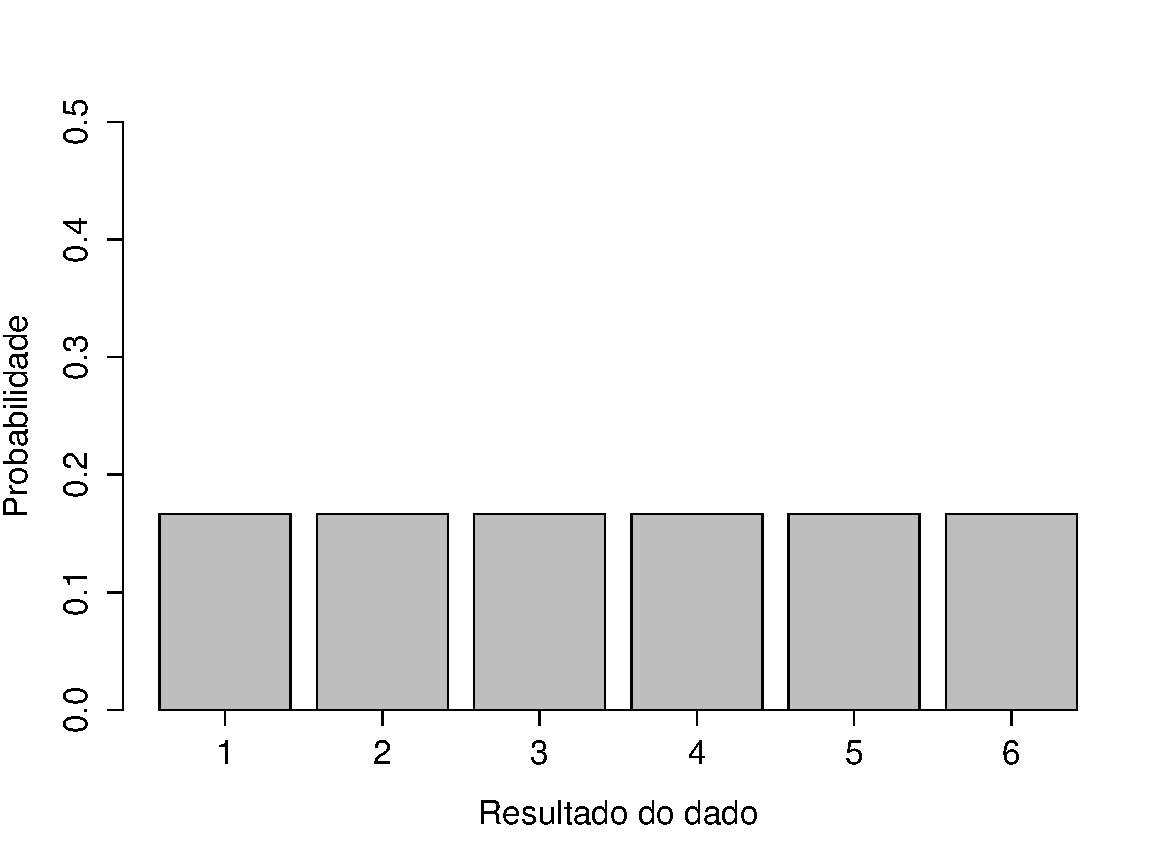
\includegraphics[scale=0.5]{uniforme-discreta}\protect\caption{\label{fig:prob1}Histograma de um dado}
\end{centering}
\end{figure}

No eixo $x$ temos os possíveis resultados do dado, ou seja, inteiros de 1 até 6. No eixo $y$ temos a probabilidade de cada resultado igual a $\frac{1}{6}$. Esta é uma \textbf{distribuição uniforme discreta}. O histograma apresenta os valores da variável no eixo $x$ e a probabilidade no eixo $y$. Entretanto, pode ser interessante olhar para a distribuição de probabilidade em sua forma acumulada, e não na forma de densidade como no histograma. 

\begin{figure}[H]
\begin{centering}
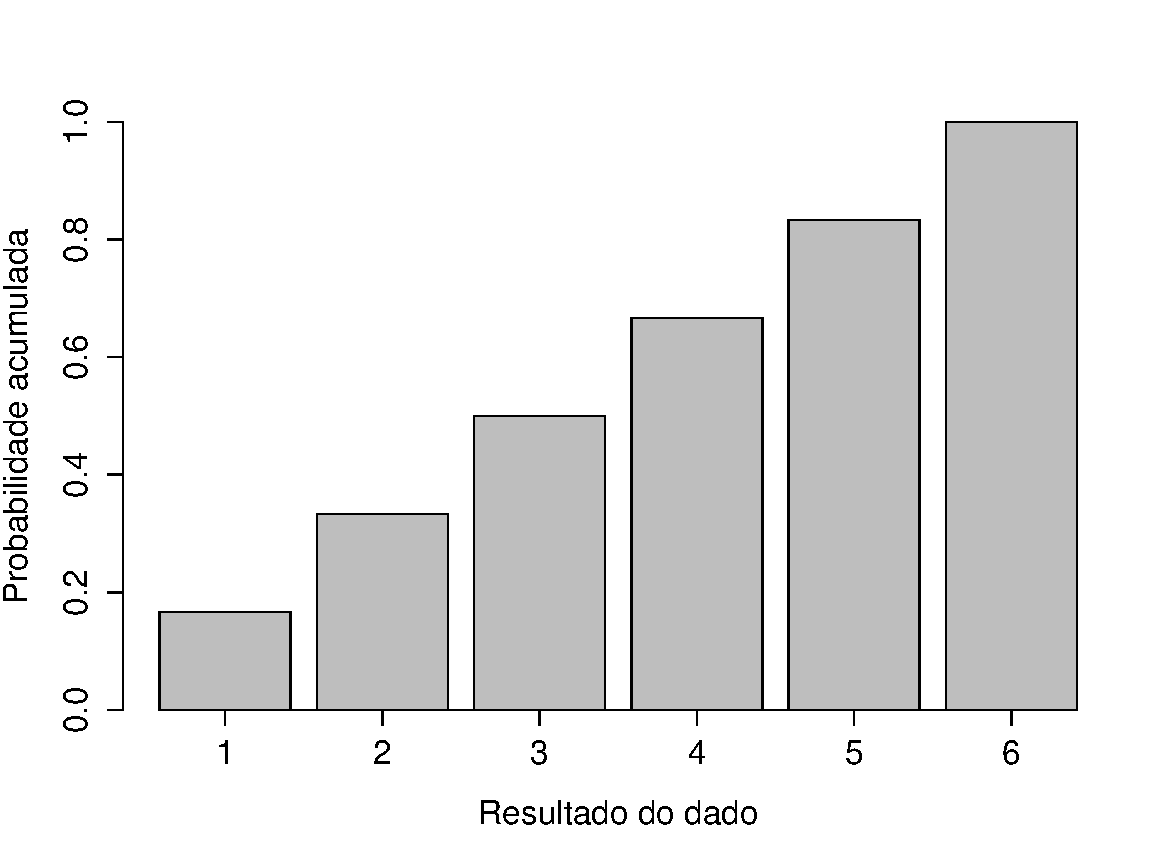
\includegraphics[scale=0.5]{uniforme-discreta-acumulada}\protect\caption{\label{fig:prob2}Distribuição acumulada de um dado}
\end{centering}
\end{figure}

A figura \ref{fig:prob2} mostra a mesma distribuição da figura \ref{fig:prob1}, porém em sua forma acumulada. No caso, a função acumulada em 4, por exemplo, representa a probabilidade de tirarmos um número menor ou igual a 4 no dado, $p(x\leq4)$. Observe que a distribuição acumulada termina onde a probabilidade assume o valor 1, ou $100\%$. Isto é o mesmo que dizer que com $100\%$ de chance tiraremos um número menor ou igual a 6 no dado, o que é verdade. No caso discreto, a distribuição acumulada terá sempre esta forma de escada, e o histograma poderá ser representado na forma de barras (fig. \ref{fig:prob1}).


Podemos escrever a distribuição do dado como uma fórmula matemática, no caso da densidade:

\begin{equation}
f(x)=p(x)=\frac{1}{6},~~~x\in [1,2,3,4,5,6]
\end{equation}

No caso da função acumulada:

\begin{equation}
F(x)=p(X\leq x)=\frac{1}{6}x,~~~x\in [1,2,3,4,5,6]
\end{equation}

Por convensão, usamos $f$ minúsculo para a função densidade e $F$ maiúsculo para a função acumulada. Além disso, o $X$ maiúsculo representa a variável aleatória do dado, e o $x$ minúsculo representa uma realização da mesma. Podemos escrever $p(X\leq 3)=\frac{1}{2}$, por exemplo. 

Por último, é interessante calcular a média e a variância das distribuições de probabilidade. A média é uma medida de \textbf{tendência central} e a variância mede a \textbf{dispersão} em torno da média. 

\begin{itemize}
\item média $=E[X]=\sum_{i=1}^n p_i x_i$
\item variância $=\sigma^2(X)=\sum_{i=1}^n p_i (x_i-E[X])^2$
\end{itemize}

onde, $p_i$ é a probabilidade do resultado $i$ acontecer. No caso da distribuição do dado esta probabilidade é igual a $\frac{1}{6}$ para todo $i$.

No caso do dado, a média e a variância são iguais a $3.5$ e $2.9$ respectivamente. Entretanto, a variância é uma medida difícil de interpretar. Imagine que estamos diante de uma distribuição de potência, a variância será medida então em potência ao quadrado. Para voltarmos para potência basta calcular o \textbf{desvio padrão}, que é a raiz quadrada da variância.\\



\textbf{\textit{Distribuições Continuas}}

Uma distribuição é contínua se seu domínio for contínuo. A mais conhecida das distribuições contínuas é a distribuição normal, seu histograma é apresentado na figura \ref{fig:prob3} e sua distribuição acumulada na figura \ref{fig:prob4}. 


\begin{figure}[H]
\begin{centering}
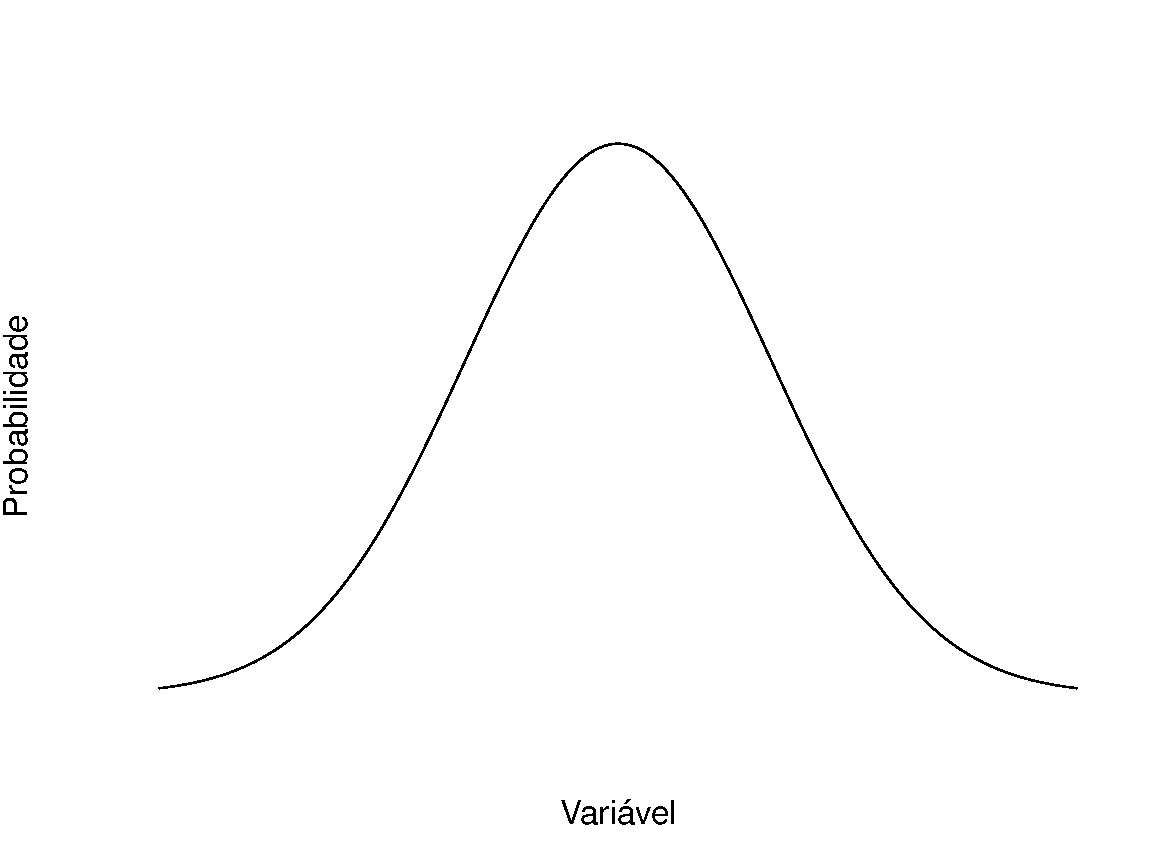
\includegraphics[scale=0.5]{histograma-normal}\protect\caption{\label{fig:prob3}Distribuição normal}
\end{centering}
\end{figure}

\begin{figure}[H]
\begin{centering}
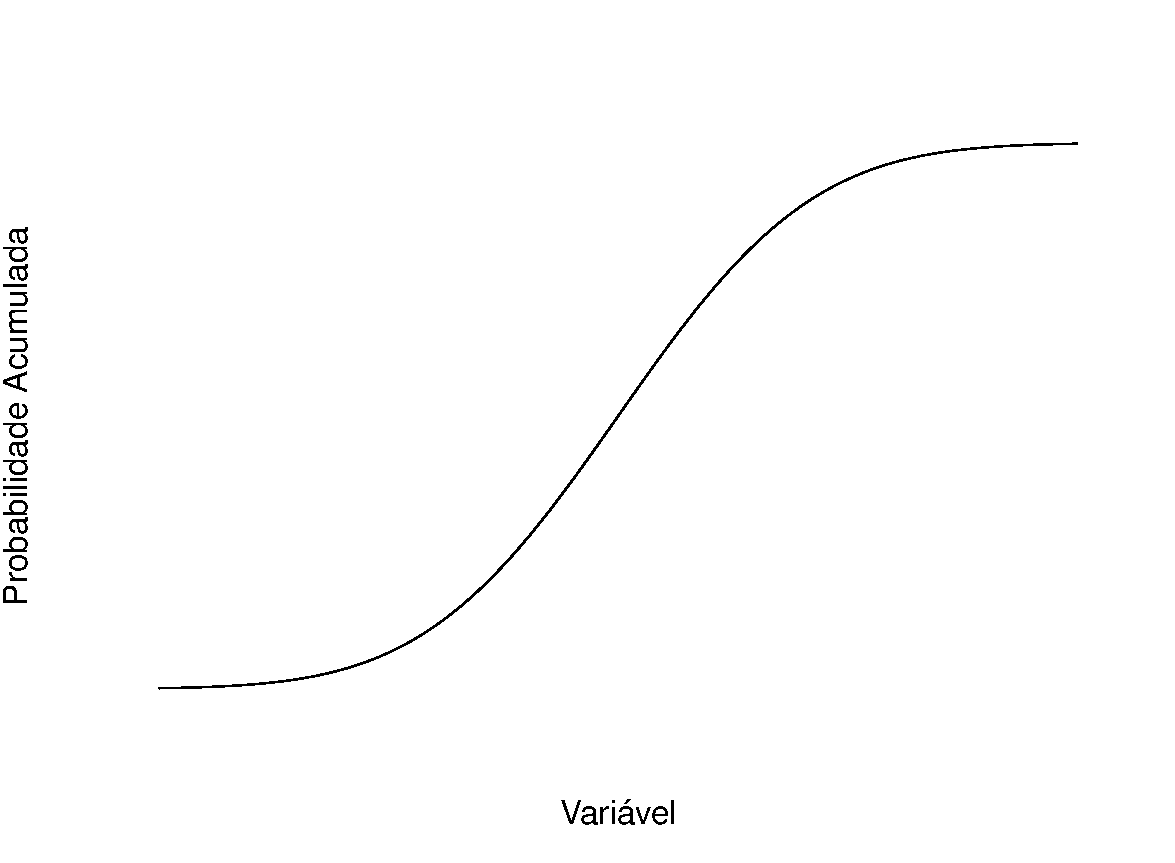
\includegraphics[scale=0.5]{histograma-normal-acumulada}\protect\caption{\label{fig:prob4}Distribuição normal acumulada}
\end{centering}
\end{figure}

O histograma de uma distribuição contínua não pode mais ser desenhado na forma de barras, e a distribuição acumulada não terá mais a forma de escada. Entretanto, a interpretação é muito semelhante à do caso discreto. Como uma distribuição contínua tem infinitos pontos no domínio, falar da probabilidade de ocorrência de um ponto isolado perde o sentido, pois esta probabilidade será igual a zero. O mais usual é falar da probabilidade de intervalos, por exemplo, a probabilidade de $x$ estar entre 1 e 2. 

Assim como no caso discreto, podemos representar as distribuições contínuas com uma fórmula, no caso da normal:

\begin{equation}
f(x)=\frac{1}{\sqrt{2 \pi \sigma^2}} e^{-\frac{(x-\mu)^2}{2\sigma^2}}
\end{equation}

A fórmula da distribuição acumulada da normal não é conhecida, entretanto, ela já foi toda tabelada e podemos utiliza-la sem problemas. Observe que na fórmula da normal temos os parâmetros $\mu$ e $\sigma^2$, que são respectivamente a média e a variância da distribuição. Portanto, se uma certa variável é normal e conhecemos sua média e sua variância, conhecemos também toda a distribuição desta variável.

Para calcular a média e a variância de uma distribuição contínua temos que calcular uma soma de infinitos elementos, por isto, o somatório é substituido pela integral.

\begin{itemize}
\item média $=\mu_X =E[X]=\int_{-\infty}^{\infty} xf(x)dx$
\item variância $=\sigma^2_X=\int_{-\infty}^{\infty} (x-E[X])^2 f(x)dx$  \end{itemize}
%\\

\textbf{\textit{Quantis}}

Uma fórma interessante de olhar para uma distribuição é separando-a em \textbf{quantis}. Quantis são pontos no domínio da distribuição acumulada que separam a mesma em intervalos iguais. Por exemplo, suponha que dividimos uma distribuição em quatro quantis\footnote{A divisão em quatro quantis é conhecida como quartil.}, a probabilidade de um elemento do domínio estar em um destes quantis é de $25\%$, e um mesmo elemento nunca estará em dois quantis ao mesmo tempo. 

Para ilustrar, suponha uma distribuição que assume os valores inteiros $[1,1,4,6,7,11,12,12]$. O primeiro quantil será $[1,1]$; o segundo será $[4,6]$, o terceiro será $[7,11]$ e o quarto será $[12,12]$. O segundo quartil, também chamado de mediana, divide a amostra no meio. A mediana é uma medida de tendência central assim como a média.

Quantis são muito úteis quando queremos estudar partes separadas das distribuições. Imagine uma distribuição de geração de um parque eólico, se queremos ver quais são os $5\%$ piores cenários de geração do nosso parque, basta separar a distribuição em 100 quantis e pegar os primeiros 5.
